\definecolor{Sail}{rgb}{0.643,0.819,0.976}
En este capítulo se abordarán los diferentes tipos de incertidumbre de medición y se explicará cómo identificar sus fuentes. Posteriormente, se revisará la importancia del certificado de calibración y su relación con la trazabilidad de las mediciones. A continuación, se definirán las fuentes de incertidumbre específicas que se consideran al calibrar los anemómetros de ultrasonido dentro del túnel de viento. Finalmente, se presentará el modelo teórico aplicado para la evaluación de la incertidumbre de medición. Este enfoque permitirá una comprensión integral de los aspectos que influyen en la precisión y fiabilidad de las mediciones realizadas en el contexto de los sensores de viento.

\section{Incertidumbre de la medición}\label{sec:tipos_incertidumbre}

La incertidumbre en la medición es una característica inherente a cualquier proceso de medición y se refiere a la duda sobre el resultado de una medición. Esta incertidumbre puede surgir de diversas fuentes, como las limitaciones del instrumento de medición, las condiciones ambientales o el método de medición empleado. Para identificar las fuentes de incertidumbre, se puede utilizar el diagrama de Ishikawa (diagrama de pescado) mostrado en la Figura \ref{fig:diagramaPescado}.

\begin{figure}[H]
    \centering
    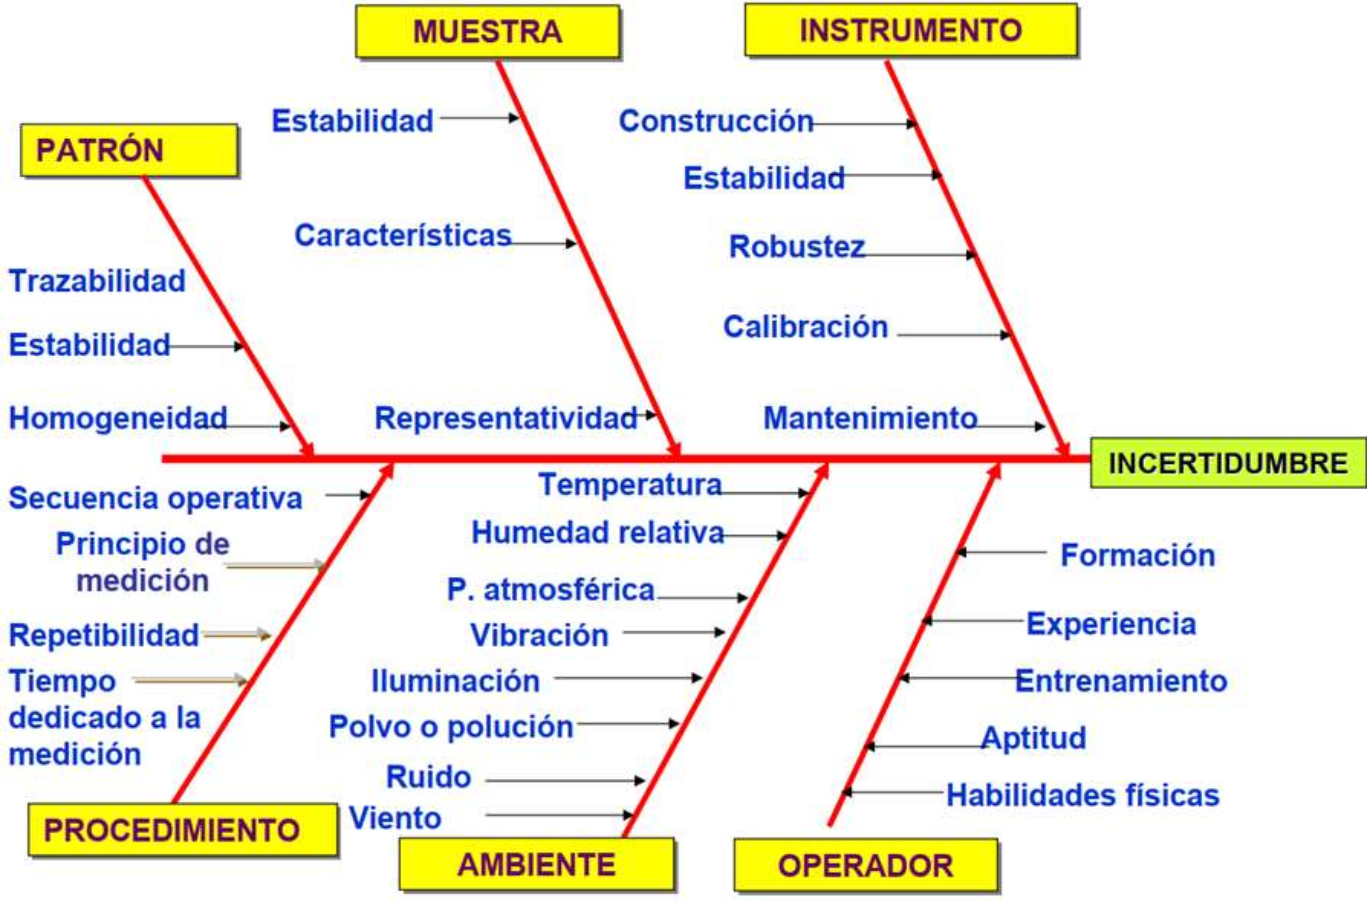
\includegraphics[width=0.8\linewidth]{Figuras/calculoIncertidumbre/diagramaPescado.png}
    \caption{Diagrama de las fuentes que producen incertidumbre en la medición de un mensurando.}
    \label{fig:diagramaPescado}
\end{figure}

Existen dos tipos principales de incertidumbre: la incertidumbre de tipo A y la incertidumbre de tipo B. La incertidumbre de tipo A se evalúa mediante métodos estadísticos y se basa en datos experimentales. A partir de una serie de observaciones de una cantidad $X_{i}$, se obtiene el promedio (ecuación \ref{eq:promedioDeObservaciones}), el desvío estándar (ecuación \ref{eq:desvioEstandarDeObservaciones}) y la incertidumbre estándar (ecuación \ref{eq:incertidumbreEstandarDeObservaciones}).


\begin{equation}
    \centering
    \bar{x} = \frac{1}{n}\sum_{i=1}^{n} x_{i}
    \label{eq:promedioDeObservaciones}
\end{equation}

\begin{equation}
    \centering
    \sigma = \sqrt{\frac{1}{n-1} \sum_{i=1}^{n} (x_i - \bar{x})^2}
    \label{eq:desvioEstandarDeObservaciones}
\end{equation}

\begin{equation}
    \centering
    u(\bar{x}) = \frac{\sigma}{\sqrt{n}}
    \label{eq:incertidumbreEstandarDeObservaciones}
\end{equation}

La incertidumbre de tipo B se basa en conocimientos previos y no en datos experimentales directos. Esta puede derivarse de información contenida en manuales, certificados de calibración o la experiencia previa con el instrumento de medición. Normalmente, se especifica un entorno $\Delta = \frac{B-A}{2}$ definido como su incertidumbre expandida. Luego, para obtener la incertidumbre estándar, se divide por un número que depende de la función de distribución asumida. Para una distribución rectangular (la más usual), se divide por $\sqrt{3}$; para una distribución triangular, se divide por $\sqrt{6}$; y para una distribución de media cuadrática (RMS), donde las fuentes de incertidumbre son idénticas y aditivamente independientes, se divide por $\sqrt{2}$.

La combinación de las incertidumbres de tipo A y tipo B da lugar a la incertidumbre combinada, que proporciona una medida más completa de la incertidumbre total asociada a una medición. Generalmente, se elabora un presupuesto de incertidumbre (\textit{uncertainty budget}) a partir de todas las fuentes identificadas, con el fin de obtener una visión detallada y precisa. La incertidumbre combinada, definida en la ecuación \ref{eq:incertidumbreCombinadaGral}, puede ser ampliada mediante un factor de cobertura, el cual se determina utilizando la distribución t de Student. Esta distribución de probabilidad ajusta el intervalo de confianza deseado en función del tamaño de la muestra y del número de grados de libertad. Los grados de libertad efectivos, representados en la ecuación \ref{eq:gradosDelibertadEfectivos}, representan el número de valores en un cálculo estadístico que son libres de variar. Esta ampliación de la incertidumbre se conoce como incertidumbre expandida, la cual se muestra en la ecuación \ref{eq:incertidumbreExpandida}, proporcionando un intervalo alrededor del resultado de la medición con una alta probabilidad de contener el valor verdadero del mensurando.

\begin{equation}
    \centering
    u_c = \sqrt{\sum_{i=1}^{n} (c_i \cdot u_i)^2}
    \label{eq:incertidumbreCombinadaGral}
\end{equation}

\begin{equation}
    \centering
    V_{ef} = \frac{u_c^4}{\sum_{i=1}^{n} \frac{u_i^4}{v_i}}
    \label{eq:gradosDelibertadEfectivos}
\end{equation}



\begin{equation}
    \centering
    U = k \cdot \sqrt{\sum_{i=1}^{n} (c_i \cdot u_i)^2}
    \label{eq:incertidumbreExpandida}
\end{equation}

%%%%%%%%%%%%%%%%%%%%%%%%%%%%%%%%%%%%%%%%%%%%%%%%%%%%%%%%%%%%%%%%%%%%%%%%%%%%%%%%%%%%%%%%%%%%%%%%%%%%%%%%%%%%%%%%%%%%%%%%
%%%%%%%%%%%%%%%%%%%%%%%%%%%%%%%%%%%%%%%%%%%%%%%%%%%%%%%%%%%%%%%%%%%%%%%%%%%%%%%%%%%%%%%%%%%%%%%%%%%%%%%%%%%%%%%%%%%%%%%%
\section{Calibración y trazabilidad}\label{sec:trazabilidad}

La calibración es el proceso mediante el cual se compara un instrumento de medición contra un instrumento estándar de referencia para asegurar su precisión. Este proceso se realiza en dos etapas: primero, se establece una relación entre los valores medidos y las incertidumbres proporcionadas por los estándares de medición; luego, se utiliza esta información para obtener resultados precisos de medición. Es importante no confundir la calibración con el ajuste del instrumento, que es un proceso diferente.

Para expresar la calibración se emiten certificados de calibración donde, en los puntos donde fue calibrado, se informa una función o tabla de corrección que se debe aplicar a las lecturas del instrumento,  lo que contribuye a mejorar la exactitud de las mediciones. Otro aspecto crucial que se debe informar en el certificado es la incertidumbre de corrección, la cual es una componente fundamental de la incertidumbre total de la medición.

El instrumento estándar también cuenta con estos parámetros en su propio certificado de calibración y son necesarios para completar el presupuesto de incertidumbre de la medición del instrumento bajo calibración (IBC), asegurando que todas las posibles fuentes de incertidumbre sean consideradas y cuantificadas.

La calibración es esencial para mantener la fiabilidad y trazabilidad a los estándares primarios. En la Figura \ref{fig:trazabilidadMetrologica} se muestra cómo, a partir de un patrón internacional, se calibra un patrón nacional tomando como referencia la incertidumbre del patrón internacional. De esta forma, en sentido descendente, se tienen incertidumbres cada vez mayores hasta llegar al equipo de medición. Por otro lado, en sentido inverso, la trazabilidad es una propiedad de un resultado de medida por la cual dicho resultado puede relacionarse con un valor de referencia, nacional o internacional, a través de una cadena ininterrumpida y documentada de calibraciones, donde cada una contribuye a la incertidumbre de la medición.

\begin{figure}[H]
    \centering
    \includegraphics[width=0.8\linewidth]{Figuras/calculoIncertidumbre/trazabilidadMetrologica.png}
    \caption{Trazabilidad metrológica.}
    \label{fig:trazabilidadMetrologica}
\end{figure}

%%%%%%%%%%%%%%%%%%%%%%%%%%%%%%%%%%%%%%%%%%%%%%%%%%%%%%%%%%%%%%%%%%%%%%%%%%%%%%%%%%%%%%%%%%%%%%%%%%%%%%%%%%%%%%%%%%%%%%%%
\section{Fuentes de incertidumbre}\label{sec:fuentesDeIncertidumbre}
En particular se va a considerar las fuentes de incertidumbre debidas a:
\begin{itemize}
    \item El sensor bajo calibración.
    \item El sensor patrón de referencia.
    \item El túnel de viento.
\end{itemize}

En la tabla \ref{tab:fuenteIncert} se detallan las fuentes de incertidumbre que se evaluarán en el presupuesto de incertidumbre para cada punto de viento configurado. En la segunda columna se nombran las fuentes y en la tercera columna se define cada una. Luego, cada incertidumbre se clasifica según el tipo, en función de cómo fue determinada. En la quinta columna se especifica el tipo de distribución probabilística. Finalmente, en la última columna se detalla el factor de normalización por el cual se debe dividir para obtener la incertidumbre estándar de cada fuente.

\newcommand{\descCalibracion}{Incertidumbre especificada  en su certificado de calibración.}
\newcommand{\descAjusteCalibracion}{Desvío estándar del ajuste lineal con los datos discretos del certificado de calibración}
\newcommand{\descResolucionInstrumento}{Menor cambio detectable.}
\newcommand{\descRepetibilidad}{Desvío estándar de la media aritmética de las mediciones.}
\newcommand{\descHisteresis}{Diferencia entre los valores de mediciones realizadas en los ciclos ascendente y descendente.}
\newcommand{\descFactorBloqueo}{Incertidumbre asociada al factor de bloqueo que se define como la relación entre el área transversal del túnel de viento y el área efectiva del anemómetro, proyectada en el plano transversal.}
\newcommand{\descHomogeneidad}{Variación espacial del flujo de aire dentro del túnel.}
\newcommand{\descAjusteHomogeneidad}{Desvío estándar del ajuste lineal con los datos discretos del certificado de homogeneidad.}
\newcommand{\descEstabilidad}{Variación temporal del flujo de aire dentro del túnel.}
\newcommand{\descAjusteEstabilidad}{Desvío estándar del ajuste lineal con los datos discretos del certificado de estabilidad.}
\newcommand{\descFactorCalib}{Incertidumbre asociada al factor de calibracion que proporciona la relación entre las condiciones en la posición de medición de referencia y las condiciones en la posición del IBC.}

\begin{table}[H]
\centering
\fontsize{9}{8}\selectfont
\begin{tblr}{
    colspec = {Q[c,1.1cm] Q[c,1.2cm] Q[c,6cm] Q[c,0.8cm] Q[c,1.9cm] Q[c,2.1cm]},
    cells = {c}, % Centra todas las celdas por defecto
    row{1} = {Sail}, % Aplica el estilo "Sail" a la primera fila
    cell{1}{1} = {c=2}{}, % La celda en la fila 1, columna 1 se extiende a dos columnas
    cell{2}{1} = {r=6}{}, % La celda en la fila 2, columna 1 se extiende a seis filas
    cell{8}{1} = {r=5}{}, % La celda en la fila 8, columna 1 se extiende a cinco filas
    cell{13}{1} = {r=4}{}, % La celda en la fila 13, columna 1 se extiende a tres filas
    vlines, % Añade líneas verticales entre todas las columnas
    hline{1-2,8,13,17} = {-}{}, % Añade líneas horizontales completas en las filas 1-2, 8, 13 y 17
    hline{3-7,9-12,14-16} = {2-6}{}, % Añade líneas horizontales parciales en las filas 3-7, 9-12 y 14-15
}
Fuentes de Incertidumbre    &                                   & Descripción               & Tipo  & Distribución de probabilidad & Factor de normalización \\
Patrón                      & Calibración                       & \descCalibracion          & B                          &  N                           &  2                      \\
                            & Ajuste de calibración         & \descAjusteCalibracion    & A                           & N                            &  1                      \\
                            & Resolución del instrumento    & \descResolucionInstrumento& B                           & R                            &  $\sqrt{3}$                      \\
                            & Repetibilidad                     & \descRepetibilidad        & A                           & N                            & $\sqrt{n}$, n muestras                      \\
                            & Histéresis                        & \descHisteresis           & B                          &  R                           & $\sqrt{3}$                       \\
                            & Factor de bloqueo             & \descFactorBloqueo        & B                          & RMS                             & 1                       \\
Túnel de viento             & Homogeneidad                      & \descHomogeneidad         & B                          & R                            & $\sqrt{3}$                       \\
                            & Ajuste de la homogeneidad     & \descAjusteHomogeneidad   & A                          & N                            & 1                       \\
                            & Estabilidad                       & \descEstabilidad          & B                           & R                            & $\sqrt{3}$                        \\
                            & Ajuste de la estabilidad      & \descAjusteEstabilidad    & A                          & N                            & 1                       \\
                            & Factor de calibración                          & \descFactorCalib              & B                          & RMS                            & 1\\
IBC                         & Resolución del Instrumento    & \descResolucionInstrumento& B                          & R                             & $\sqrt{3}$                        \\
                            & Repetibilidad                     & \descRepetibilidad        & A                          & N                            & $\sqrt{n}$, n muestras                        \\
                            & Histéresis                        & \descHisteresis           & B                           & R                            & $\sqrt{3}$                        \\
                            & Factor de bloqueo             & \descFactorBloqueo        & B                          & RMS                             & 1                       \\
\end{tblr}
\caption{Fuentes de incertidumbre evaluadas para el presupuesto de incertidumbre de un anemotro bajo calibracion en el tunel de viento del SMN.}
\label{tab:fuenteIncert}
\end{table}
%%%%%%%%%%%%%%%%%%%%%%%%%%%%%%%%%%%%%%%%%%%%%%%%%%%%%%%%%%%%%%%%%%%%%%%%%%%%%%%%%%%%%%%%%%%%%%%%%%%%%%%%%%%%%%%%%%%%%%%%

\section{Modelo teórico de medición}\label{sec:modelo_teoricos}

El modelo de medición utilizado para calcular la incertidumbre se muestra en la ecuación \ref{eq:ModeloIncertidumbre}. Este modelo se basa en una comparación, donde se obtiene la corrección del mensurando bajo calibración a partir de la diferencia de medición en un punto determinado y bajo condiciones ambientales controladas, entre un patrón calibrado y el instrumento bajo calibración.

\begin{equation}
    CV_{IBC} = \overbrace{V_{p} + CV_{p}}^{V_{ref}} - V_{IBC}
    \label{eq:ModeloIncertidumbre}
\end{equation}
donde se define:

\begin{itemize}
    \item $V_{IBC}$ representa el valor de viento medido con el anemómetro bajo calibración.
    \item $CV_{IBC}$ representa la corrección del anemómetro bajo calibración.
    \item $V_{p}$ representa el valor de viento medido con el anemómetro patrón.
    \item $CV_{p}$ representa la corrección de viento del anemómetro patrón, obtenida a partir de su certificado de calibración.
\end{itemize}

A partir de la ecuación \ref{eq:ModeloIncertidumbre} y tomando en cuenta las fuentes de incertidumbre, definidas en la tabla \ref{} se realiza el calculo de la incertidumbre combinada de la corrección, como la suma de los cuadrados de las incertidumbres estándar de cada fuente, como se muestra en la ecuación \ref{eq:incertidumbreCombinada}.

\begin{equation}
    u^{2}(CV_{IBC}) = u^{2}(V_{ref})+u^{2}(V_{IBC})+u^{2}(\text{túnel de Viento})
    \label{eq:incertidumbreCombinada}
\end{equation}
donde se define:

\begin{itemize}
    \item $u^{2}(CV_{IBC})$ es la incertidumbre estándar de la corrección del anemómetro bajo calibración.
    \item $u^{2}(V_{ref})$ representa la suma de todas las fuentes de incertidumbre estándar debidas al patrón de referencia.
    \item $u^{2}(V_{IBC})$ representa la suma de todas las fuentes de incertidumbre estándar debidas al anemómetro bajo calibración.
    \item $u^{2}(\text{túnel de Viento})$ es la contribución de incertidumbre estándar referida al túnel de viento, quien se encarga de generar condiciones de velocidad y dirección de viento.
\end{itemize}


